\chapter[Задача распознавания эмоций по звучащей речи]{Задача распознавания эмоций\\по звучащей речи}

\chapter{Классификация эмоций}
Одной из главных проблем в исследованиях, связанных с определением эмоционального состояния диктора по голосу, является отсутствие чёткого определения эмоции. При формализации этого понятия возникают сложности в силу многообразия психологических моделей эмоциональных процессов. Подход к классификации эмоций влияет на процесс аннотирования -- разметки аудиовизуального эмоционально окрашенного контента. 

Для формализации эмоциональных данных необходимо сформировать полноценную классификацию эмоциональных состояний, от которой в том числе напрямую зависит процесс аннотирования -- сопоставления инофрмативных признаков, полученных из речи диктора с определенными эмоциями и аффективными состояниями.

Сегодня широко используются три подхода : дискретная и многомерная модели, а также гибридная.

\section{Дискретная модель эмоциональной сферы}
Дискретный подход основан на выделении фундаментальных (базовых) эмоций, сочетания которых порождают разнообразие эмоциональных явлений. Разные авторы называют разное число таких эмоций -- от двух до десяти. П.~Экман на основе изучения лицевой экспрессии выделяет пять базовых эмоций: гнев, страх, отвращение, печаль и радость. Первоначальная версия 1999 года также включала <<удивление>> \cite{Ekman1972, Ekman1992}. Р.~Плутчик \cite{Plutchik1980} выделяет восемь базисных эмоций, деля их на четыре пары, каждая из которых связана с определенным действием: страх, уныние, удивление и т.~д. На рисунке \ref{fig:emo-atlas} представлена схема классификации эмоций, предложенная П.~Экманом. 

На сегодняшний день концепция существования базовых эмоций ставится под сомнение. Теория встречает ряд концептуальных проблем, таких как, например, эмпирическое определение набора базовых эмоций или критерии синхронизации эмоциональных реакций. Однако, многие решения в области автоматического детектирования эмоций основаны на дискретной модели эмоциональной сферы. Например, решение компании Affectiva \cite{Affectica}.

\begin{figure}[H]
	\centering
	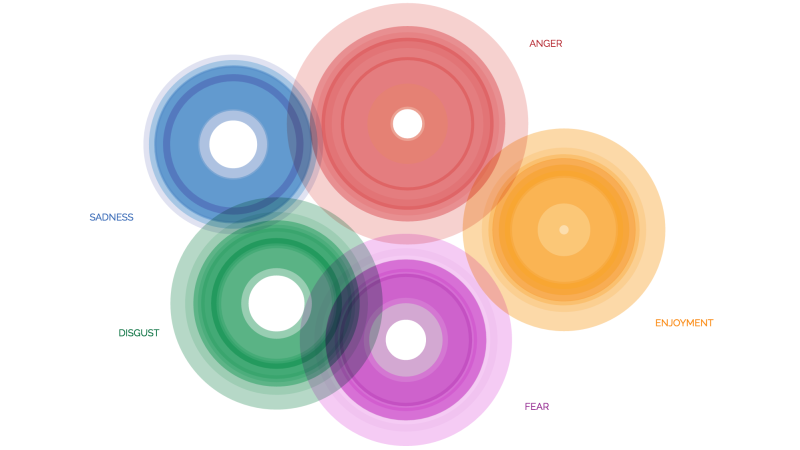
\includegraphics[width=\linewidth]{assets/emo-atlas.png}
	\caption{Атлас эмоций, предложенный П.~Экманом}
	\label{fig:emo-atlas}
\end{figure}

\section{Многомерная модель эмоциональной сферы}
Многомерная модель представляет собой эмоции в координатном многомерном пространстве. В качестве её источника рассматривают идею В. Вундта о том, что многогранность чувств
человека можно описать с помощью трёх измерений: удовольствие~-~неудовольствие, расслабление~-~напряжение, возбуждение~-~успокоение. Вундт заключил, что эти измерения охватывают все разнообразие эмоциональных состояний \cite{Вундт1984}. Данные для этой теории были получены с помощью метода интроспекции.

Эмоциональная сфера представляется как многомерное пространство, образованное некоторым
количеством осей координат. Оси задаются полюсами первичных характеристик эмоций. Отдельные эмоции -- это точки, местоположение которых в <<эмоциональном>> пространстве определяется степенью выраженности этих параметров.

Один из примеров описываемого подхода -- модель Дж. Рассела. В ней водится двумерный базис, в котором каждая эмоция характеризуется знаком (\textit{valence}, валентность) и интенсивностью (\textit{arousal}, активацией). Измерение валентности отражает то,
насколько хорошо человек ощущает себя на уровне субъективного переживания от максимального неудовольствия до максимального удовольствия. Измерение активации связано с
субъективным чувством энергии и ранжируется в диапазоне от дремоты до бурного возбуждения. Такой подход используется, например, в датасете RECOLA \cite{RECOLA}.

Аналогично вопросу о количестве эмоций в дискретной модели, вопрос о количестве измерений остаётся открытым. Использование только двух критикуется на том основании, что они не позволяют устанавливать различия между отдельными эмоциональными состояниями (например, страх, гнев, ревность, презрение и др. имеют отрицательную валентность и высокую активацию).

\section{Гибридная модель эмоциональной сферы}
Гибридная модель представляет собой комбинацию дискретной и многомерной модели. Согласно этой классификации, в отдельной области $n$~-мерного эмоционального пространства различия между эмоциями могут определяться в терминах измерений, имеющих отношение к этой области. Эмоции могут быть сопоставимы по измерениям внутри и вне категорий, и каждая категория может иметь свои отличительные признаки \cite{Russell2003}. Примером такой модели являются <<Песочные часы эмоций>>, предложенные Камбрией, Ливингстоном, Хуссейном \cite{hourglass}. Каждое измерение характеризуется шестью уровнями
силы, с которой выражены эмоции. Данные уровни обозначаются набором из двадцати четырёх эмоций. Поэтому совершенно любая эмоция может рассматриваться как и фиксированное состояние, так и часть пространства, связанная с другими эмоциями нелинейными отношениями. 
\begin{figure}[H]
	\centering
	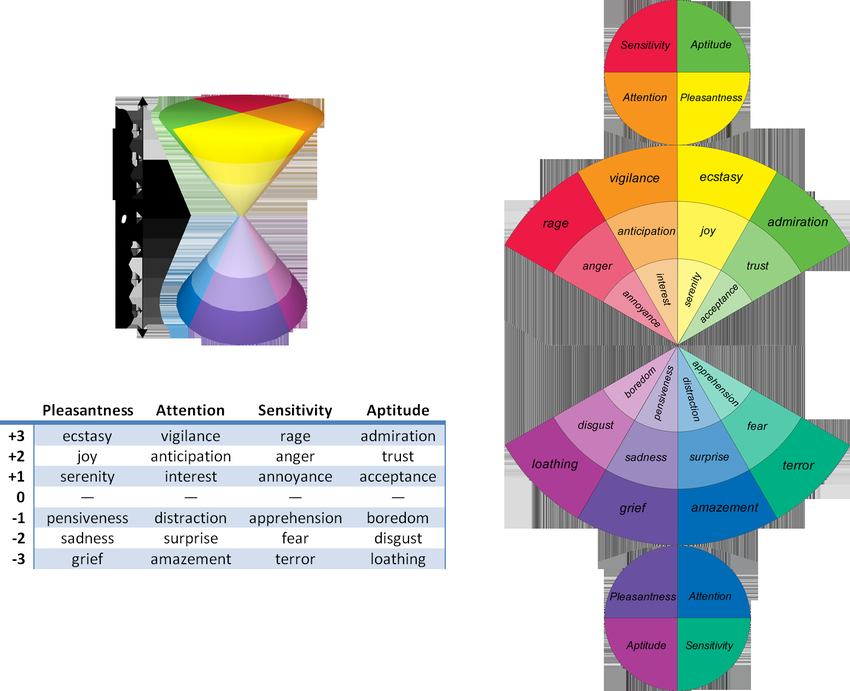
\includegraphics[width=0.9\linewidth]{assets/hourglass.png}
	\caption{<<Песочные часы эмоций>>}
	\label{fig:hourglass}
\end{figure}

Выбор подхода от цели. Многомерные модели позволяют избежать проблемы существования  некоторых слов в каких-то языках, в то время как в других может не быть слов для описания этих эмоций. Это делает процесс аннотирования культурно-зависимым. Тем не менее разные аннотаторы дают разные оценки выраженности валентности или активации, поэтому в целях упрощения модели для некоторых задач больше подходит дискретная модель.

\chapter{Автоматическое распознавание речи}
\section{Речеобразование и классификация звуков}
Реечвой аппарат человека представлен на рисунке \ref{fig:voice-anatomy}. Акустически процесс речеобразования образования состоит из нескольких независимых этапов.~\cite{Фант1964} Первый -- возникновение звука в артикуляторном тракте, которое, в свою очередь, может быть реализовано либо голосовым, либо шумовым, либо импульсным источником. Второй -- формирование возбуждённого звука и его излучение в пространство.

\begin{figure}[H]
	\centering
	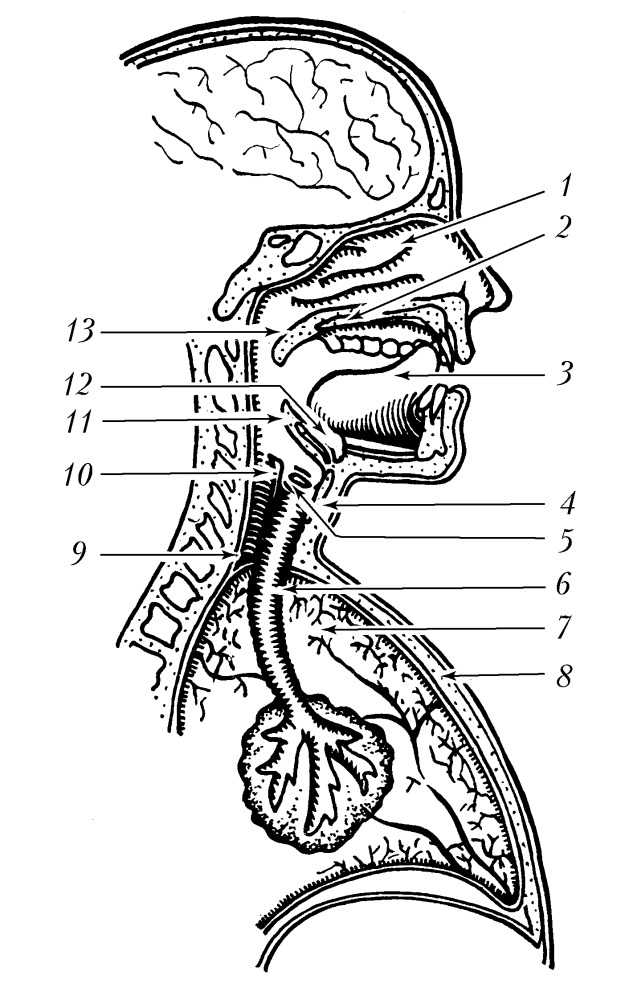
\includegraphics[width=0.45\linewidth]{assets/voice.jpg}
	\caption{Речевой аппарат человека: \textit{1~--~носовая полость, 2~--~твёрдое нёбо, 3~--~язык, 4~--~щитовидный хрящ, 5~--~голосовые связки, 6~--~трахея, 7~--~лёгкое, 8~--~грудина, 9~--~пищевод, 10~--~кольцеобразный хрящ, 11~--~надгортанье, 12~--~подъязычная кость, 13~--~мягкое нёбо.}}
	\label{fig:voice-anatomy}
\end{figure}

Речевые звуки можно классифицировать в зависимости от источника возникновения. Классификация приведена в таблице \ref{tab:sounds}.


\begin{table}[H]
	\caption{Классификация речевых звуков}
	\label{tab:sounds}
	\begin{tabular}{|p{0.08\textwidth}p{0.15\textwidth}|p{0.35\textwidth}|p{0.15\textwidth}|p{0.1\textwidth}|}
		\hline
		\multicolumn{2}{|p{0.1\textwidth}|}{\textsc{раздел}} & \textsc{артикуляция} & \textsc{источник} & \textsc{пример} \\ \hline \hline
		\multicolumn{2}{|p{0.1\textwidth}|}{гласные} & не создаётся существенных препятствий & голосовой & \textsc{{[}а{]}, {[}у{]}} \\ \hline
		\multicolumn{1}{|p{0.08\textwidth}|}{\multirow{2}{*}{смычные}}& аффрикаты & размыкание смычки происходит плавно & голосовой совместно с шумовым & \textsc{{[}ч{]}, {[}ц{]}} \\ \cline{2-5} 
		\multicolumn{1}{|p{0.15\textwidth}|}{согласные} & взрывные & нёбная занавеска поднята, и воздух проходит в ротовую полость, а размыкание смычки происходит резко и напоминает взрыв & звонкие -- голосовой с импульсным, глухие -- импульсный & \textsc{{[}п{]}, {[}т{]}, {[}к{]} , {[}б{]}, {[}д{]}, {[}г{]}} \\ \hline
		\multicolumn{2}{|p{0.3\textwidth}|}{сонорные согласные} & без участия турбулентного потока воздуха в голосовом тракте & голосовой & \textsc{{[}й’{]}, {[}л{]}} \\ \hline
		\multicolumn{2}{|p{0.2\textwidth}|}{щелевые (фрикативные) согласные} & артикуляторы подходят близко друг к другу, но не смыкаются полностью, в результате чего в ротовой полости происходят турбулентные колебания воздуха, создающие заметный шум & звонкие -- голосовой совместно с шумовым, глухие -- шумовой & \textsc{{[}ж{]}, {[}ж':{]}, {[}ш{]}, {[}ш':{]}} \\ \hline
	\end{tabular}
\end{table}

%Голосовые складки колеблются при продувании через них потока
%воздуха под действием эффекта Бернулли \cite{Фланаган1968}. Частота колебаний голосовых
%складок называется основным тоном. Частота колебаний голосовых складок при обычной речи находится в пределах 60-180 Гц для мужчин, 160-350 Гц для женщин и 200-650
%Гц для детей (указанные границы ориентировочные)\cite{Фланаган1968}. Форма
%импульсов голосового источника в основном и определяет тембр голоса.

\section{Слуховая система}

Для задачи автоматического распознавания речи важно изучение слухового анализатора, поскольку неадекватная обработка сигнала может привести к потере полезных признаков. 

Периферическую слуховую систему представляют как последовательно включенные наружное, среднее и внутреннее ухо (рисунок \ref{fig:hearing}).

\begin{figure}[H]
	\centering
	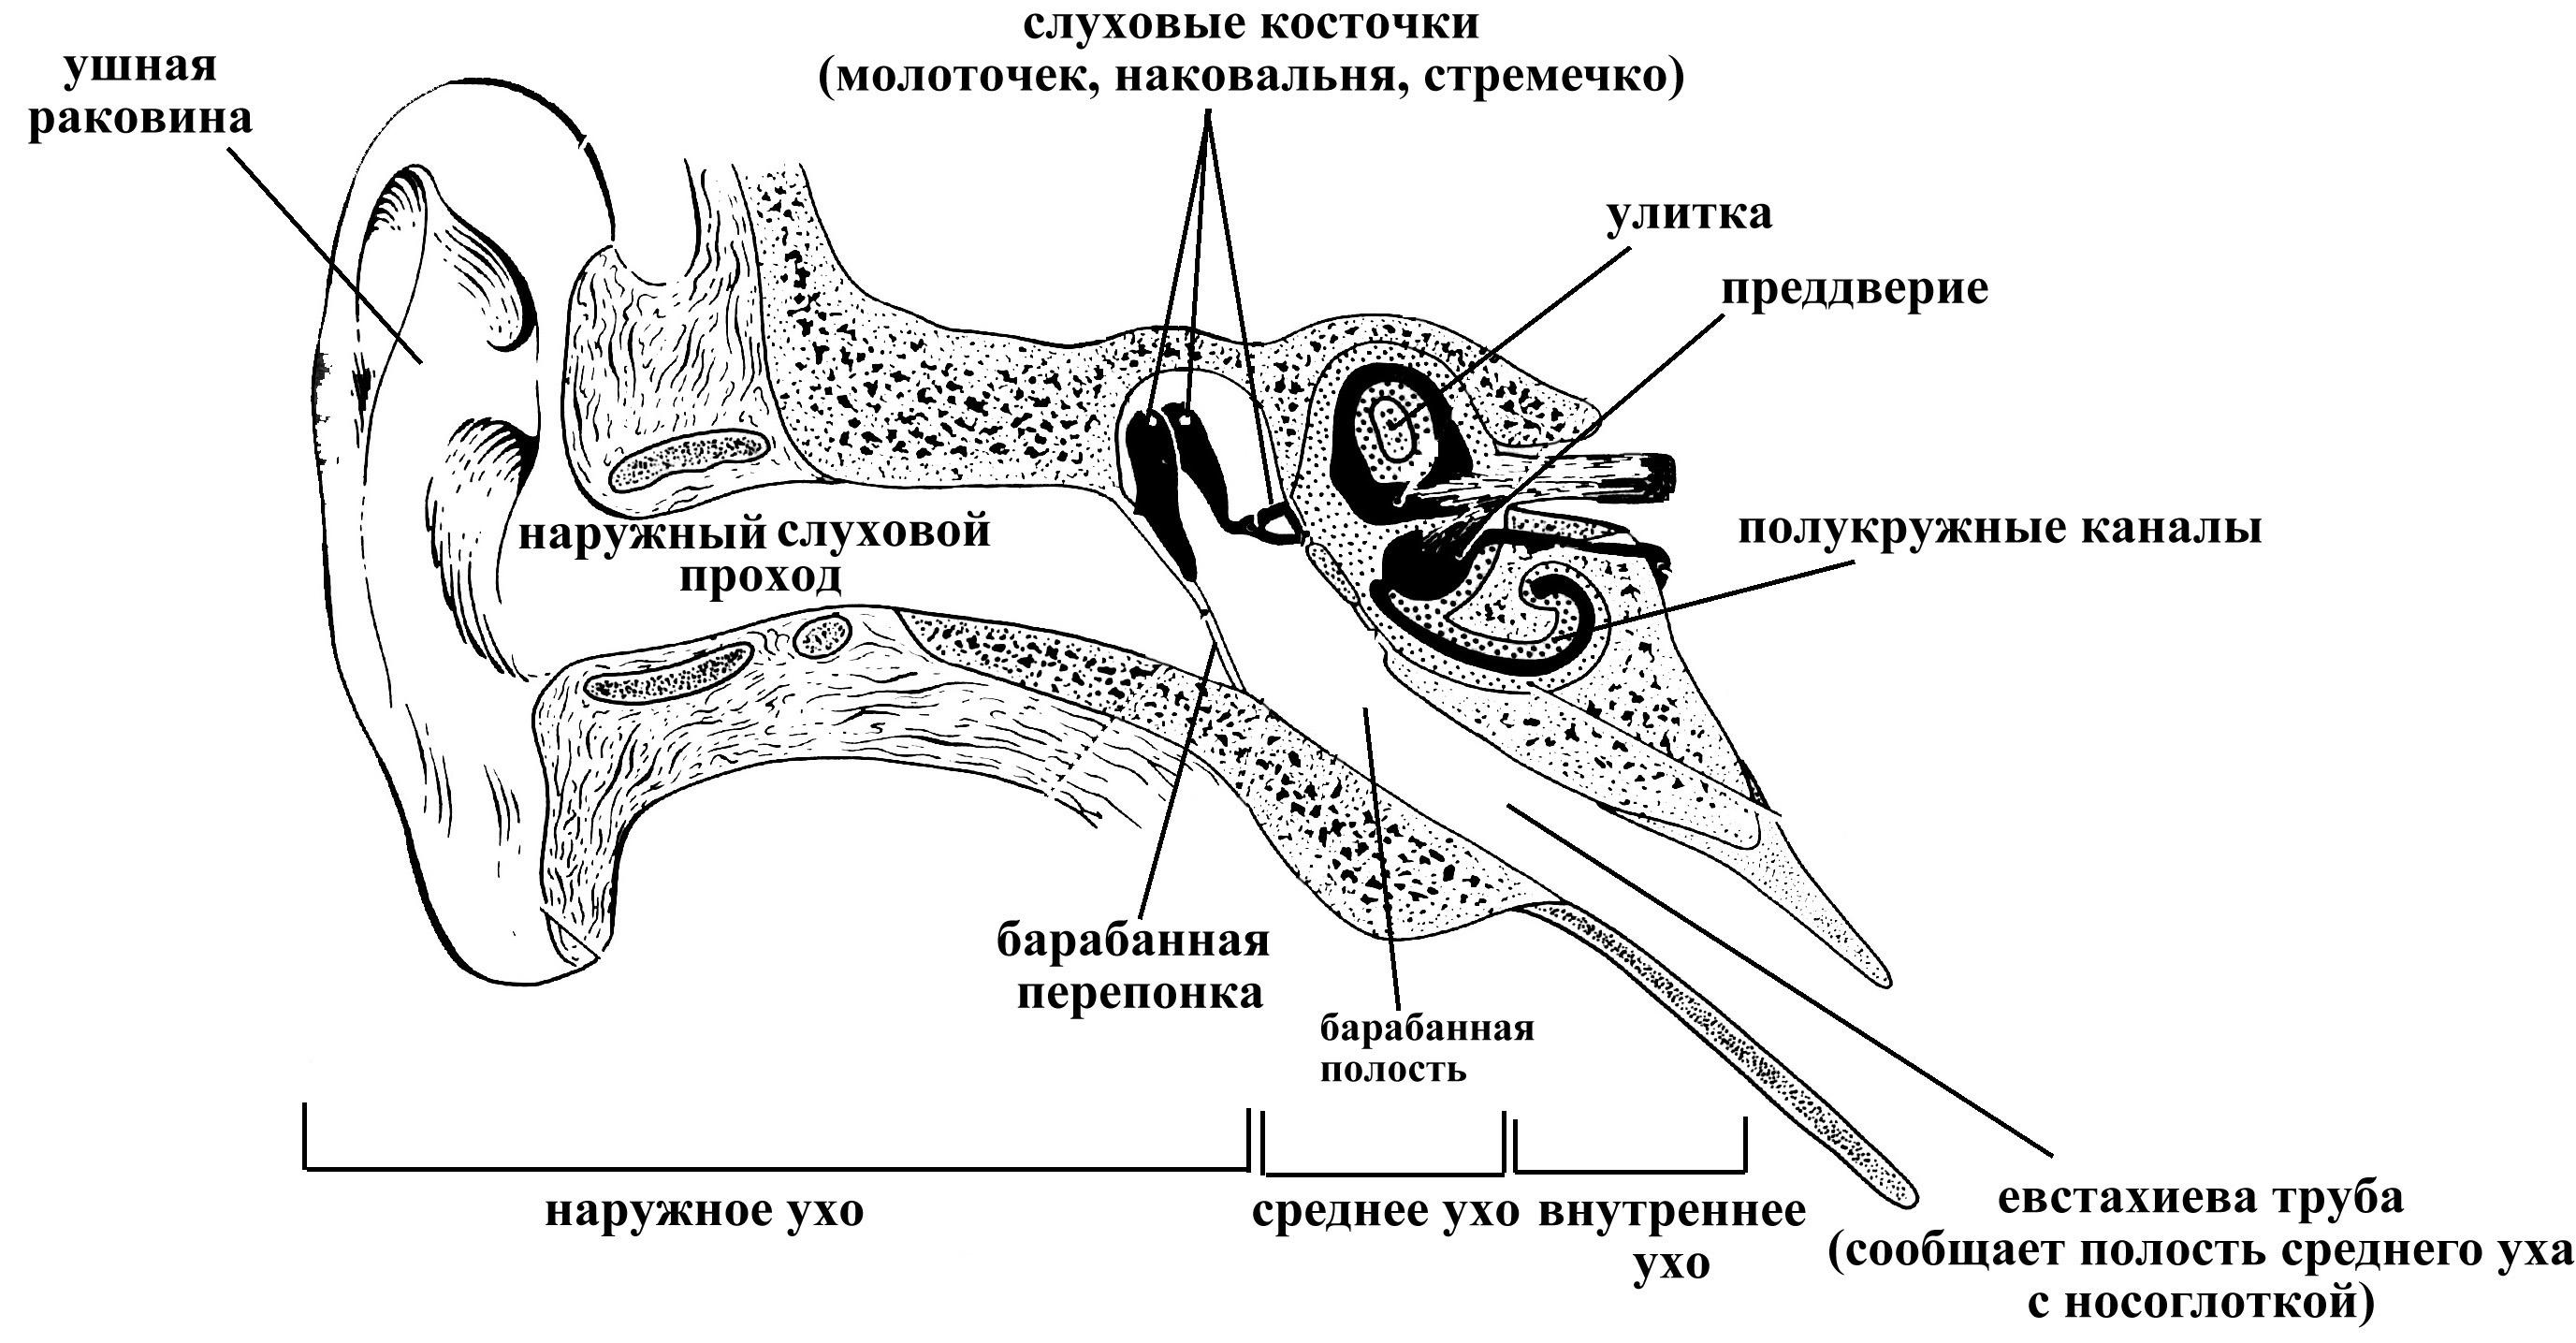
\includegraphics[width=0.9\linewidth]{assets/hear.jpg}
	\caption{Слуховая система человека}
	\label{fig:hearing}
\end{figure}

Система каналов улитки является акустическим фильтром низких частот. Таким образом, высокочастотные составляющие слышимого звука, а также продуктов отоакустической эмиссии затухают в вестибулярном и тимпанальном каналах и не достигают круглого окна. Частота запирания ниже 14 кГц\cite{Дидковский2014}. 

\subsection{Восприятие высоты звука}
О восприятии звука на разных частотах даёт представление следующий эксперимент \cite{Алдошина1999}. Слушателю предъявляют гармонический сигнал и просят выставить частоту второго сигнала так, чтобы на его субъективный взгляд она была в два раза выше или ниже, чем частота предъявленного. Восприятие высоты звука зависит от его интенсивности, поэтому, для получения однозначных результатов, интенсивность стимулов во втором эксперименте фиксируют в 40 дБ. Из полученных результатов следует, что слуховая система склонна рассматривать низкочастотные компоненты речи более подробно, чем высокочастотные -- начиная с 1000 Гц, шкалы можно считать близкими к логарифмическим. 
\subsection{Восприятие громкости звука}

Громкость -- это субъективная оценка интенсивности звука. Ощущение громкости зависит не только от частоты, но и от длительности звукового стимула. Для количественной оценки абсолютной громкости была принята специальная единица сон. Громкость в 1 сон – это громкость синусоидального звука с частотой 1000 Гц и уровнем 40 дБ относительно звукового давления $2 \cdot 10^{-5}$ Па.

Количественно зависимость воспринимаемой громкости звука (в сонах) и его звукового давления может быть представлена в виде \ref{eq:son}:

\begin{equation}\label{eq:son}
	S = Cp^{0.6},
\end{equation}
где $$
\chapter{Информативные признаки, характеризующие речь}

Выделение информативного набора признаков, коррелированных с эмоциональным состоянием, оказывает значительное влияние на эффективность автоматического детектирования эмоций.
